% Candidate titles (not used):
% 1. Short-Sequence Cardiac Progression Prediction on MIMIC-IV: Sequence Models Versus Temporal Feature Gradient Boosting
% 2. Predicting Worsening Cardiac Progression From Six-Visit ICU Trajectories Using Explicit Temporal Descriptors
% 3. Longitudinal ICU Cardiac Progression Modeling: An Empirical Comparison of Transformers and Temporally Engineered Boosting
\documentclass[conference]{IEEEtran}

\usepackage{amsmath,amssymb}
\usepackage{booktabs}
\usepackage{multirow}
\usepackage{url}
\usepackage{cite}
\usepackage{balance}
\usepackage{graphicx}
\usepackage{tikz}
\usetikzlibrary{arrows.meta,positioning,shapes.geometric}

\title{Longitudinal Cardiac Progression Prediction From ICU Records: Comparing Sequence Models and Temporal Feature Gradient Boosting}

\author{\IEEEauthorblockN{H~M~Akshay,
Hemanth~Kumar~K,
Shreya~G,
Venkat~Baba~Yemineni,
and Padmasree~N}
\IEEEauthorblockA{RV Institute of Technology and Management (RVITM)\\
Visvesvaraya Technological University (VTU), Bengaluru, India}}

\begin{document}
\maketitle

\begin{abstract}
Cardiovascular deterioration is a longitudinal process, yet many predictive models summarize a patient with a single encounter and therefore underuse trajectory information available in intensive-care records. This paper studies binary prediction of worsening cardiac progression from longitudinally ordered ICU stays in MIMIC-IV version~2.1. We construct a cardiac cohort from ICD diagnosis codes, aggregate vital and laboratory measurements into 59 features per stay, form fixed-length six-visit sequences, and define worsening using a Cardiac Severity Index (CSI) increase of more than 10\% between consecutive stays, with in-hospital mortality as a fallback label for terminal observations. Two modeling tracks are compared: (i)~end-to-end sequence classifiers (bidirectional LSTM with attention, bidirectional GRU, and a Transformer encoder) and (ii)~gradient-boosting models trained on explicit temporal descriptors of change, variability, and acceleration, followed by isotonic calibration and validation-based threshold selection. On a held-out test set of 5{,}289 sequences (16.9\% positive), a reproduced Transformer baseline achieved F1~$=$~$0.6319$ and ROC-AUC~$=$~$0.9168$, whereas a calibrated soft-voting ensemble of HistGradientBoosting, LightGBM, and XGBoost achieved F1~$=$~$0.7334$, precision~$=$~$0.7226$, recall~$=$~$0.7444$, and ROC-AUC~$=$~$0.9462$. For short ICU trajectories, explicit temporal feature engineering with calibrated boosting improved the precision--recall operating point relative to larger sequence models in this internal evaluation. The study is retrospective research and is not intended for diagnosis or clinical decision-making.
\end{abstract}

\begin{IEEEkeywords}
MIMIC-IV, cardiac progression, longitudinal electronic health records, temporal feature engineering, gradient boosting, Transformer, ICU risk prediction.
\end{IEEEkeywords}

\section{Introduction}
Cardiovascular diseases remain a leading cause of global mortality and disability~\cite{roth2020gbd}. In critical care, deterioration is rarely instantaneous: vital signs, cardiac biomarkers, and metabolic laboratories evolve across successive intensive-care unit (ICU) encounters. Models that encode only a single snapshot can miss the direction, speed, and instability of that evolution. Longitudinal electronic health records (EHRs) therefore motivate progression-oriented prediction rather than static disease classification~\cite{choi2016doctorai,harutyunyan2019mimic}.

Prior clinical machine-learning work has achieved strong results for mortality, decompensation, phenotype labeling, and next-visit code prediction using recurrent and attention-based architectures~\cite{harutyunyan2019mimic,choi2016doctorai,choi2016retain}. Parallel work shows that gradient-boosted trees remain competitive for structured clinical features~\cite{chen2016xgboost,ke2017lightgbm}. What remains less clear for short ICU trajectories is whether end-to-end sequence models automatically learn the clinically relevant temporal structure, or whether making change, variability, and acceleration explicit yields a better precision--recall tradeoff under class imbalance.

This paper addresses that question on a cardiac cohort derived from MIMIC-IV~2.1~\cite{johnson2023mimic,johnson2022mimiciv21}. We formulate worsening progression prediction as a patient-trajectory classification task over chronologically ordered ICU stays, compare bidirectional recurrent and Transformer sequence models with a temporal-feature gradient-boosting track, and evaluate discrimination and operating-point metrics under an approximately 16.9\% positive-class prevalence. The central finding is empirical rather than architectural: on six-visit sequences, calibrated boosting over engineered temporal descriptors outperformed the strongest reproduced sequence baseline in F1 and ROC-AUC while remaining compact for CPU inference.

The main contributions are:
\begin{enumerate}
\item a reproducible formulation of binary cardiac progression prediction on MIMIC-IV~2.1 using six-visit ICU sequences with 59 features per visit and a CSI-based worsening label;
\item a controlled comparison of BiLSTM-attention, BiGRU, and Transformer sequence classifiers against HistGradientBoosting, LightGBM, XGBoost, and calibrated ensembles trained on explicit temporal descriptors;
\item quantitative evidence that, for these short sequences, temporal feature engineering with isotonic calibration and validation-tuned thresholds improved F1 from $0.6319$ to $0.7334$ and ROC-AUC from $0.9168$ to $0.9462$ relative to a reproduced Transformer baseline; and
\item an explicit audit of methodological risks---including sample-level rather than patient-disjoint splitting, label heterogeneity from mortality fallback, and proxy medication features---that constrain clinical interpretation.
\end{enumerate}

\section{Related Work}

\subsection{Cardiovascular Risk and Progression Modeling}
Classical cardiovascular risk tools emphasize long-horizon population risk using sparse baseline covariates. More recent EHR studies model recurrent heart-failure trajectories and comorbidity-conditioned progression with recurrent networks~\cite{lu2021dhtm}. Those works typically target diagnosis-onset sequences over months or years. In contrast, the present study focuses on short, high-resolution ICU stay sequences and a physiology-derived severity change label rather than administrative diagnosis recurrence alone.

\subsection{Machine Learning on Electronic Health Records}
Public critical-care databases, especially MIMIC, have enabled reproducible clinical machine learning~\cite{johnson2023mimic,harutyunyan2019mimic}. Benchmark tasks commonly include in-hospital mortality, physiologic decompensation, length of stay, and phenotype classification~\cite{harutyunyan2019mimic}. Such benchmarks demonstrate the value of longitudinal physiologic time series, but they do not directly define cardiac progression as a CSI transition between successive ICU stays. Our cohort construction and label definition are therefore complementary to standard MIMIC benchmarks.

\subsection{Temporal and Sequential Clinical Modeling}
Recurrent models such as Doctor~AI predict subsequent diagnoses and medications from visit histories~\cite{choi2016doctorai}. Attention mechanisms, including RETAIN, improve interpretability by highlighting influential visits and codes~\cite{choi2016retain}. Transformer self-attention further removed recurrence as a requirement for sequence transduction~\cite{vaswani2017attention}. These methods are well suited to longer code sequences; whether their capacity is necessary for six-step ICU trajectories with dense numeric features remains an empirical question addressed here.

\subsection{Gradient Boosting for Structured Clinical Prediction}
XGBoost and LightGBM are widely used for nonlinear tabular prediction because they capture feature interactions efficiently and train quickly relative to deep models~\cite{chen2016xgboost,ke2017lightgbm}. In clinical settings they are often paired with hand-crafted aggregates. Our temporal-feature track follows that tradition: we do not propose a new boosting algorithm, but rather evaluate whether descriptors of trajectory shape make short-sequence progression prediction more amenable to calibrated tree ensembles.

\subsection{Research Gap}
Existing work establishes strong sequential EHR models and strong tabular boosters separately. Fewer studies directly ask, under a fixed short ICU trajectory length and a progression-oriented cardiac label, whether explicit temporal descriptors plus calibrated boosting can outperform end-to-end sequence learners. That comparison---and the accompanying leakage, label, and deployment analysis---is the gap addressed by this paper.

\section{Problem Formulation}
Let patient $i$ contribute a chronologically ordered sequence of ICU-stay feature vectors
\begin{equation}
X_i = \{x_{i,1}, x_{i,2}, \ldots, x_{i,T_i}\}, \qquad x_{i,t}\in\mathbb{R}^{d},
\end{equation}
where $d=59$ in this study. A fixed-length window of $L=6$ consecutive stays is extracted (with left padding when $T_i<6$). For a window ending at stay $t$, the binary target is
\begin{equation}
y_{i,t}=
\begin{cases}
1, & \text{if } CSI_{i,t+1}>1.10\,CSI_{i,t},\\
0, & \text{otherwise,}
\end{cases}
\end{equation}
when a subsequent stay exists. For a patient's final or only stay, the implementation substitutes the hospital in-hospital mortality flag. Thus $y=1$ denotes predicted worsening progression under a heterogeneous operational definition: CSI increase for transitions and mortality for terminal observations. The learning task is to estimate $p(y=1\mid X)$ and choose a decision threshold on validation data.

\section{Materials and Methods}

\subsection{Dataset and Cohort Construction}
Experiments use the deidentified MIMIC-IV version~2.1 hospital and ICU modules~\cite{johnson2023mimic,johnson2022mimiciv21}: \texttt{patients}, \texttt{admissions}, \texttt{diagnoses\_icd}, \texttt{icustays}, \texttt{chartevents}, and \texttt{labevents}. Access to MIMIC-IV requires PhysioNet credentialing and a data-use agreement; the present analysis uses only deidentified records.

A cardiac cohort is selected using ICD-9/ICD-10 diagnosis prefixes covering ischemic heart disease, myocardial infarction, heart failure, arrhythmia, cardiomyopathy, valvular disease, hypertensive heart disease, pulmonary heart disease, and related conditions.
\textbf{[DATASET DETAIL REQUIRED: exact ICD prefix list and age criteria].}

The reported full run identified 66{,}841 cardiac subjects, 157{,}019 cardiac admissions, and 52{,}130 cardiac ICU stays before sequence construction. After preprocessing and six-visit window generation, the model-ready dataset contained 35{,}256 samples: 24{,}678 training, 5{,}289 validation, and 5{,}289 testing samples. Each split contained approximately 16.9\% positives. The held-out test set contained 896 worsening and 4{,}393 stable/improving examples.

\subsection{Feature Extraction and Preprocessing}
Vital signs are streamed from \texttt{chartevents} and laboratory values from \texttt{labevents}. Extracted variables include heart rate; systolic, diastolic, and mean blood pressure; respiratory rate; temperature; oxygen saturation; fingerstick glucose; troponin; BNP/NT-proBNP; creatinine; BUN; glucose; electrolytes; bicarbonate; hematocrit; hemoglobin; WBC; and platelets. Repeated measurements within a stay are summarized using statistics such as mean, standard deviation, and maximum. Contextual variables include age, length of stay, prior myocardial infarction, prior heart failure, prior arrhythmia, diagnosis counts, admission type, time since the previous admission, time from the first ICU stay, and visit index.

The resulting representation contains 59 features per ICU stay. Missing values are forward- and backward-filled within each patient timeline; remaining missing values are imputed with training-split feature medians, with zeros used for any residual non-finite values. A \texttt{StandardScaler} is fit on the training split only and applied to validation and test data. The final tensor has shape $(N,6,59)$.

\subsection{Cardiac Severity Index and Label Semantics}
CSI is a hand-engineered severity score derived from abnormalities in heart rate, blood pressure, troponin, BNP/NT-proBNP, oxygen saturation, creatinine, respiratory rate, and hemoglobin.
\textbf{[IMPLEMENTATION DETAIL REQUIRED: CSI weights and thresholds].}
Because CSI is not a clinically adjudicated gold standard, all progression claims in this paper refer to the operational CSI/mortality label rather than to chart-reviewed deterioration.

\subsection{Sequence Construction, Splitting, and Leakage Controls}
Patients are ordered chronologically. Sliding windows of six visits are created for patients with sufficient history; shorter histories are left-padded by repeating the earliest available row. Samples are partitioned 70\%/15\%/15\% with stratified random splitting and \texttt{random\_state=42}. Scaling uses training data only.

\paragraph{Patient-level contamination.}
The current implementation splits generated windows rather than enforcing patient-disjoint partitions. Overlapping windows from the same patient may therefore appear across splits, which can inflate apparent generalization. Results should be interpreted as an internal benchmark pending patient-disjoint and chronological evaluation.
\textbf{[TEMPORAL LEAKAGE VALIDATION REQUIRED: patient-disjoint and time-based holdout].}

\paragraph{Prediction-time leakage.}
Labels for transitional samples use $CSI_{t+1}$ relative to $CSI_t$; features for a window are constructed from stays available at prediction time within that window. Future diagnoses after the prediction point, discharge disposition beyond the label definition, and later laboratory values outside the window must not enter the feature set. Medication-count features in the current pipeline are documented as proportional proxies derived from diagnosis counts rather than from prescription tables; those proxies should be replaced with direct medication extraction in future revisions.

\subsection{Sequence Models}
Three neural baselines consume the raw $(6\times 59)$ sequence:
\begin{itemize}
\item \textbf{BiLSTM-attention:} two-layer bidirectional LSTM (hidden size 128, dropout 0.3) with attention pooling over visit representations and a fully connected classification head.
\item \textbf{BiGRU:} two-layer bidirectional GRU with the same hidden size and dropout, using the final bidirectional state as the sequence representation.
\item \textbf{Transformer encoder:} each visit is projected to $d_{\mathrm{model}}=128$; a learnable classification token is prepended; sinusoidal positional encoding is added; three encoder layers with eight heads, feed-forward width 512, and dropout 0.1 produce a sequence representation for a two-layer classification head~\cite{vaswani2017attention}.
\end{itemize}
Neural models use weighted binary cross-entropy with logits to address class imbalance, AdamW optimization, gradient clipping, validation-loss checkpointing, and early stopping. Reproduced fair-comparison runs used learning rate $3\times 10^{-4}$, batch size 128, up to 80 epochs, and patience 12. Reported neural operating thresholds in the baseline tables are $0.5$ unless otherwise stated.

\subsection{Temporal Feature Gradient Boosting}
``Temporal gradient boosting'' in this work denotes gradient boosting trained on temporally engineered tabular features; it is not a new boosting algorithm. Each $(6\times 59)$ sequence is converted into a flat descriptor vector containing the flattened sequence together with per-feature summaries: first and last values, mean, standard deviation, minimum, maximum, median, interquartile range, range, delta, coefficient of variation, slope, half-split trend, consecutive-change velocity, second-difference acceleration, total variation, and position of the last value within the observed range. A ``simple'' configuration uses 826 features; richer configurations feed HistGradientBoosting, LightGBM, and XGBoost~\cite{chen2016xgboost,ke2017lightgbm}.

Candidates are selected using validation PR-AUC. Selected models are calibrated with isotonic regression on validation predictions~\cite{niculescu2005calibration}. A decision threshold maximizing validation F1 is then frozen and applied to the test set. The soft-voting ensemble averages calibrated probabilities from HistGradientBoosting, LightGBM, and XGBoost; its documented operating threshold is $0.335$. A stacked ensemble is also evaluated. Exact tree depths, learning rates, and leaf constraints are selected by validation search.
\textbf{[IMPLEMENTATION DETAIL REQUIRED: hyperparameter grids and selected configs].}

\subsection{Evaluation Metrics}
Because positives comprise only $\approx$16.9\% of samples, accuracy alone is insufficient. We report accuracy, precision, recall (sensitivity), F1, ROC-AUC (tables: AUC), and PR-AUC / average precision (tables: AP). Precision and recall are defined with respect to the worsening class. For imbalanced progression prediction, PR curves and F1 at a validation-chosen threshold are particularly informative; ROC-AUC remains useful for ranking quality.

\subsection{Experimental Setup}
Primary neural training was performed in a GPU-enabled notebook environment; boosting models train on CPU.
\textbf{[IMPLEMENTATION DETAIL REQUIRED: hardware and library versions].}
Stratified splits use \texttt{random\_state=42}. Neural results in Table~\ref{tab:baseline-original} come from a full-run training pass; Table~\ref{tab:baseline-repro} reports a later reproduction on the identical arrays used by the boosting track and is the fair baseline for improvement claims. Confidence intervals and multi-seed means are not yet available.
\textbf{[EXPERIMENT REQUIRED: multi-seed runs and patient-level bootstrap CIs].}

\begin{figure}[t]
\centering
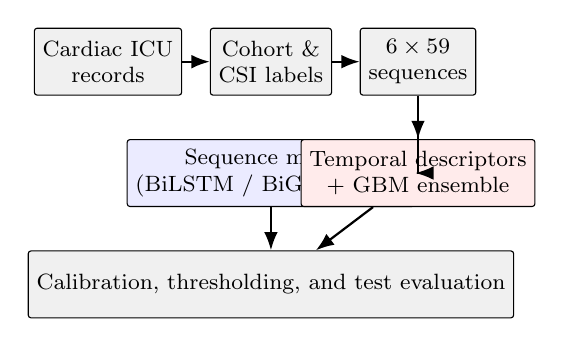
\begin{tikzpicture}[
  font=\footnotesize,
  box/.style={draw, rounded corners=1pt, align=center, inner sep=3pt, minimum height=0.85cm},
  arr/.style={-{Latex}, thick}
]
\node[box, fill=gray!12] (a) {Cardiac ICU\\records};
\node[box, right=0.35cm of a, fill=gray!12] (b) {Cohort \&\\CSI labels};
\node[box, right=0.35cm of b, fill=gray!12] (c) {$6\times 59$\\sequences};
\node[box, below=0.55cm of b, fill=blue!8, minimum width=2.6cm] (d) {Sequence models\\(BiLSTM / BiGRU / TF)};
\node[box, below=0.55cm of c, fill=red!8, minimum width=2.6cm] (e) {Temporal descriptors\\+ GBM ensemble};
\node[box, below=0.55cm of d, fill=gray!12, minimum width=5.8cm] (f) {Calibration, thresholding, and test evaluation};
\draw[arr] (a) -- (b);
\draw[arr] (b) -- (c);
\draw[arr] (c.south) |- (d.east);
\draw[arr] (c) -- (e);
\draw[arr] (d) -- (f);
\draw[arr] (e) -- (f);
\end{tikzpicture}
\caption{Overview of the dual-track pipeline: sequence models consume raw six-visit tensors, while the boosting track consumes engineered temporal descriptors.}
\label{fig:pipeline}
\end{figure}

\section{Results}

\subsection{Neural Sequence Baselines}
Table~\ref{tab:baseline-original} summarizes the original full-run sequence results at threshold $0.5$. The Transformer obtained the best accuracy, precision, F1, and ROC-AUC; BiGRU obtained the highest recall. Weighted loss produced high recall with precision near $0.48$, illustrating an aggressive alert profile at the default threshold.

\begin{table}[t]
\caption{Original full-run sequence-model results on the held-out test set (threshold $0.5$).}
\label{tab:baseline-original}
\centering
\scriptsize
\setlength{\tabcolsep}{3.5pt}
\begin{tabular}{lccccc}
\toprule
Model & Acc. & Prec. & Rec. & F1 & AUC\\
\midrule
BiLSTM-Attn & 0.8134 & 0.4712 & 0.8304 & 0.6012 & 0.9021\\
BiGRU & 0.8132 & 0.4712 & \textbf{0.8404} & 0.6038 & 0.9076\\
Transformer & \textbf{0.8198} & \textbf{0.4814} & 0.8237 & \textbf{0.6077} & \textbf{0.9096}\\
\bottomrule
\end{tabular}
\end{table}

Table~\ref{tab:baseline-repro} reports the fair reproduction on the arrays shared with the boosting experiments. The reproduced Transformer is the primary sequence baseline for subsequent comparisons.

\begin{table}[t]
\caption{Reproduced sequence baselines on the arrays used by the boosting track (threshold $0.5$).}
\label{tab:baseline-repro}
\centering
\scriptsize
\setlength{\tabcolsep}{3.5pt}
\begin{tabular}{lccccc}
\toprule
Model & Acc. & Prec. & Rec. & F1 & AUC\\
\midrule
BiLSTM-Attn & 0.8308 & 0.5003 & 0.8103 & 0.6187 & 0.9060\\
BiGRU & 0.8211 & 0.4837 & \textbf{0.8259} & 0.6101 & 0.9099\\
Transformer & \textbf{0.8399} & \textbf{0.5174} & 0.8114 & \textbf{0.6319} & \textbf{0.9168}\\
\bottomrule
\end{tabular}
\end{table}

\subsection{Temporal Feature Gradient-Boosting Results}
Table~\ref{tab:improved} reports calibrated boosting results at validation-selected thresholds. The soft-voting ensemble achieved the best F1 ($0.7334$) and tied the best ROC-AUC ($0.9462$). The stacked ensemble slightly improved accuracy, precision, and PR-AUC at the cost of lower recall and F1. Individual HistGradientBoosting, LightGBM, and XGBoost models remained close to one another, indicating that the temporal representation---not a single backend---drove most of the gain.

\begin{table}[t]
\caption{Temporal-feature gradient-boosting results on the held-out test set (validation-calibrated thresholds).}
\label{tab:improved}
\centering
\scriptsize
\setlength{\tabcolsep}{2.8pt}
\begin{tabular}{lcccccc}
\toprule
Method & Acc. & Prec. & Rec. & F1 & AUC & AP\\
\midrule
Soft vote & 0.9083 & 0.7226 & 0.7444 & \textbf{0.7334} & \textbf{0.9462} & 0.8302\\
Stacked & 0.9125 & 0.7612 & 0.7042 & 0.7316 & \textbf{0.9462} & \textbf{0.8307}\\
HistGB & \textbf{0.9126} & \textbf{0.7747} & 0.6830 & 0.7260 & 0.9434 & 0.8093\\
LightGBM & 0.9079 & 0.7332 & 0.7176 & 0.7253 & 0.9439 & 0.8153\\
XGBoost & 0.9032 & 0.6983 & \textbf{0.7545} & 0.7253 & 0.9433 & 0.8069\\
Simple (826) & 0.9102 & 0.7451 & 0.7143 & 0.7293 & 0.9450 & 0.8115\\
\bottomrule
\end{tabular}
\end{table}

Relative to the reproduced Transformer, the soft-voting ensemble improved F1 by $0.1015$ absolute and ROC-AUC by $0.0294$, while raising precision from $0.5174$ to $0.7226$ and retaining recall $0.7444$. Fig.~\ref{fig:model-comparison} summarizes that comparison. The gain is therefore not explained by simply predicting more positives.

\begin{figure}[t]
\centering
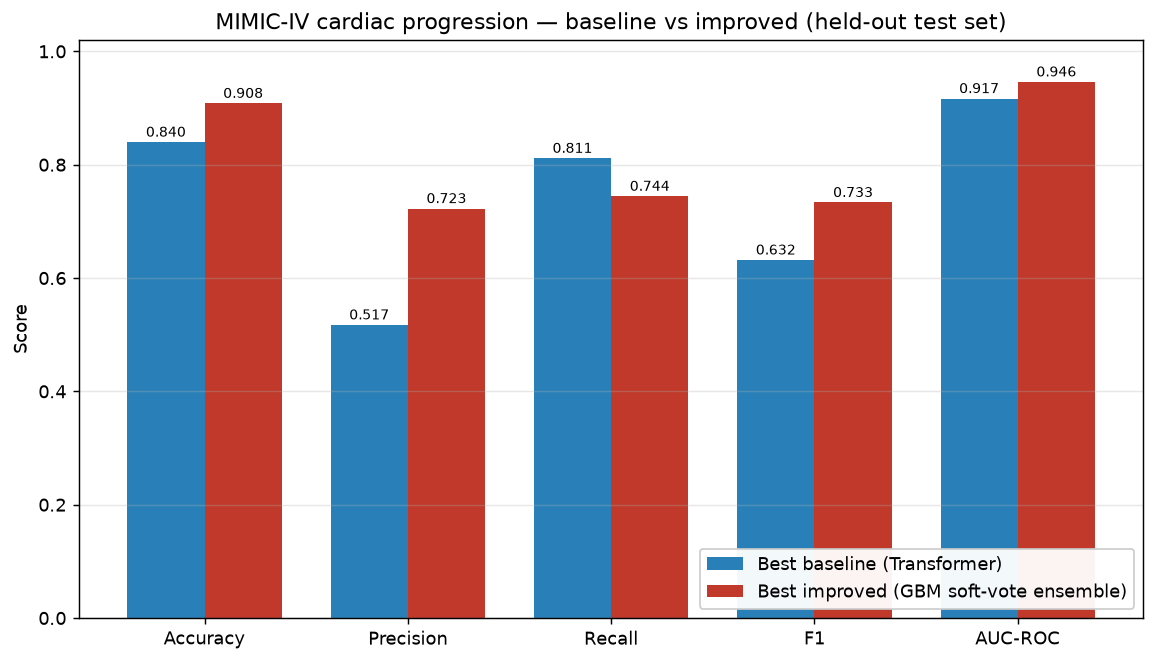
\includegraphics[width=\columnwidth]{figures/improved_model_comparison.png}
\caption{Held-out comparison of the reproduced Transformer baseline and the GBM soft-voting ensemble.}
\label{fig:model-comparison}
\end{figure}

Fig.~\ref{fig:curves} shows ROC and precision--recall curves for sequence and boosting models. Boosting curves dominate across most of the operating range.
\textbf{[FIGURE CONSISTENCY CHECK REQUIRED: regenerate curve legends from the same prediction files as the tables].}
Primary quantitative claims in this paper rely on the tables.

\begin{figure}[t]
\centering
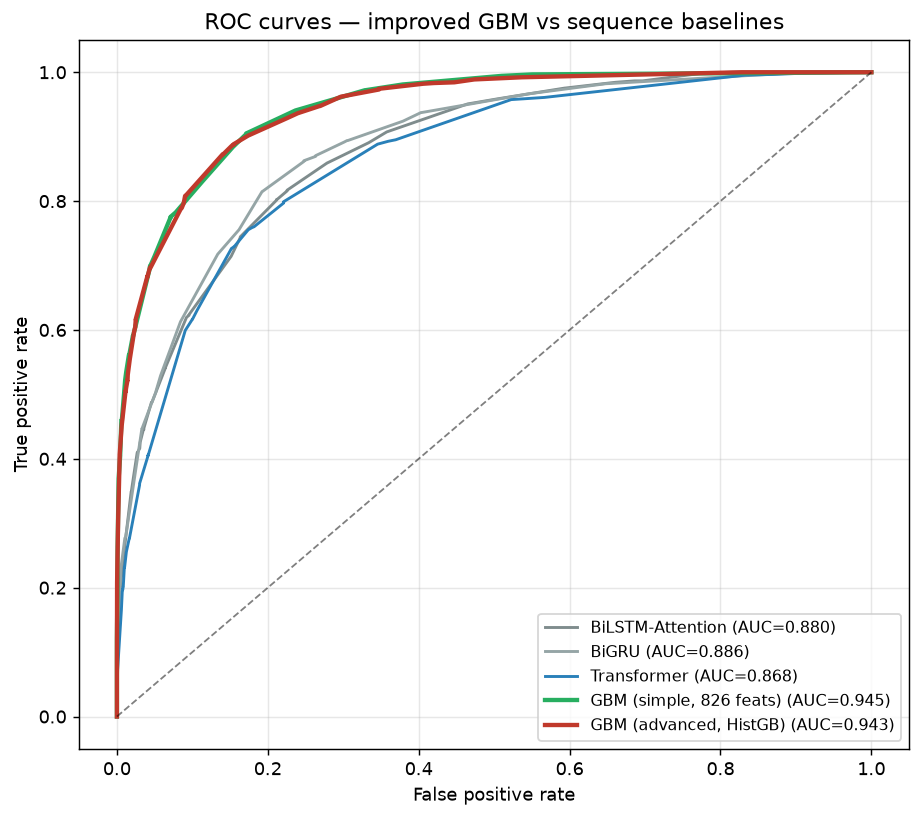
\includegraphics[width=0.49\columnwidth]{figures/improved_roc_curves.png}
\hfill
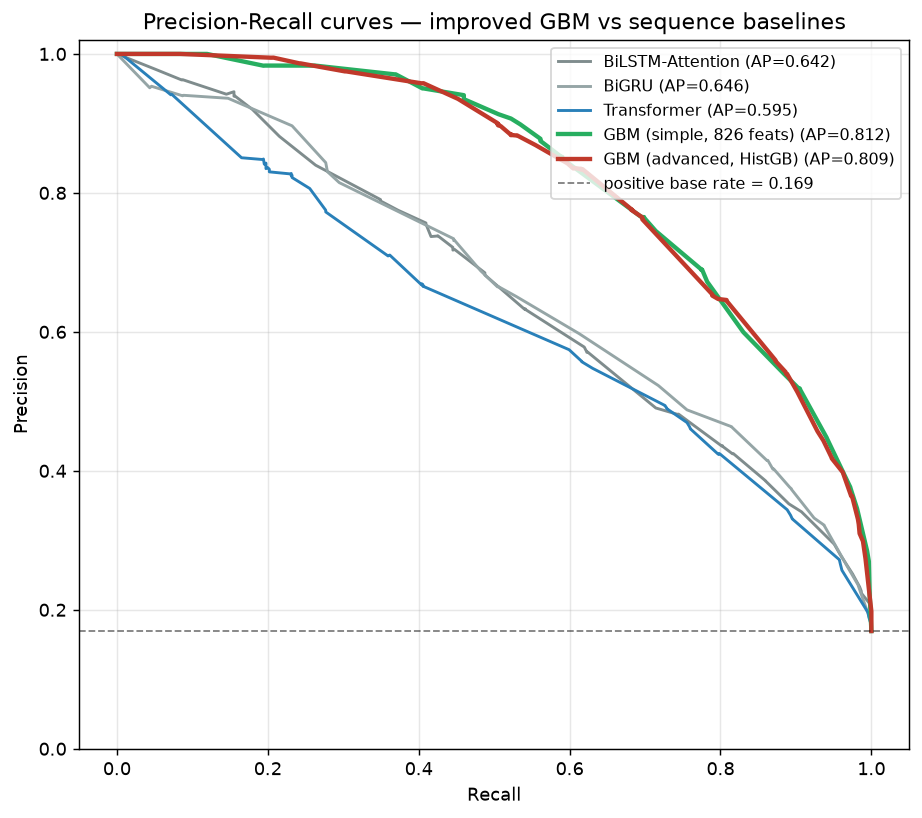
\includegraphics[width=0.49\columnwidth]{figures/improved_pr_curves.png}
\caption{ROC and precision--recall curves for sequence baselines and temporal-feature boosting models. Prefer Table metrics when legend values conflict.}
\label{fig:curves}
\end{figure}

\subsection{Error Profile and Feature Attribution}
At threshold $0.335$, the soft-voting ensemble confusion matrix on the test set counts 4{,}137 true negatives, 667 true positives, 256 false positives, and 229 false negatives (Fig.~\ref{fig:interpretability}, left). Feature-gain attributions from LightGBM highlight oxygen-saturation variability, bicarbonate, blood-pressure and heart-rate levels or variability, age, length of stay, temperature, and WBC-related descriptors among the leading signals (Fig.~\ref{fig:interpretability}, right). These associations describe model behavior; they are not causal effects and should not be interpreted as treatment guidance.

\begin{figure}[t]
\centering
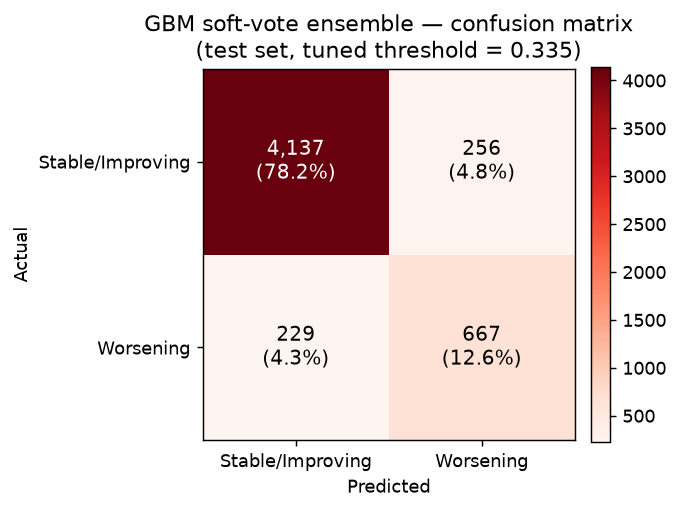
\includegraphics[width=0.49\columnwidth]{figures/improved_confusion_matrix.png}
\hfill
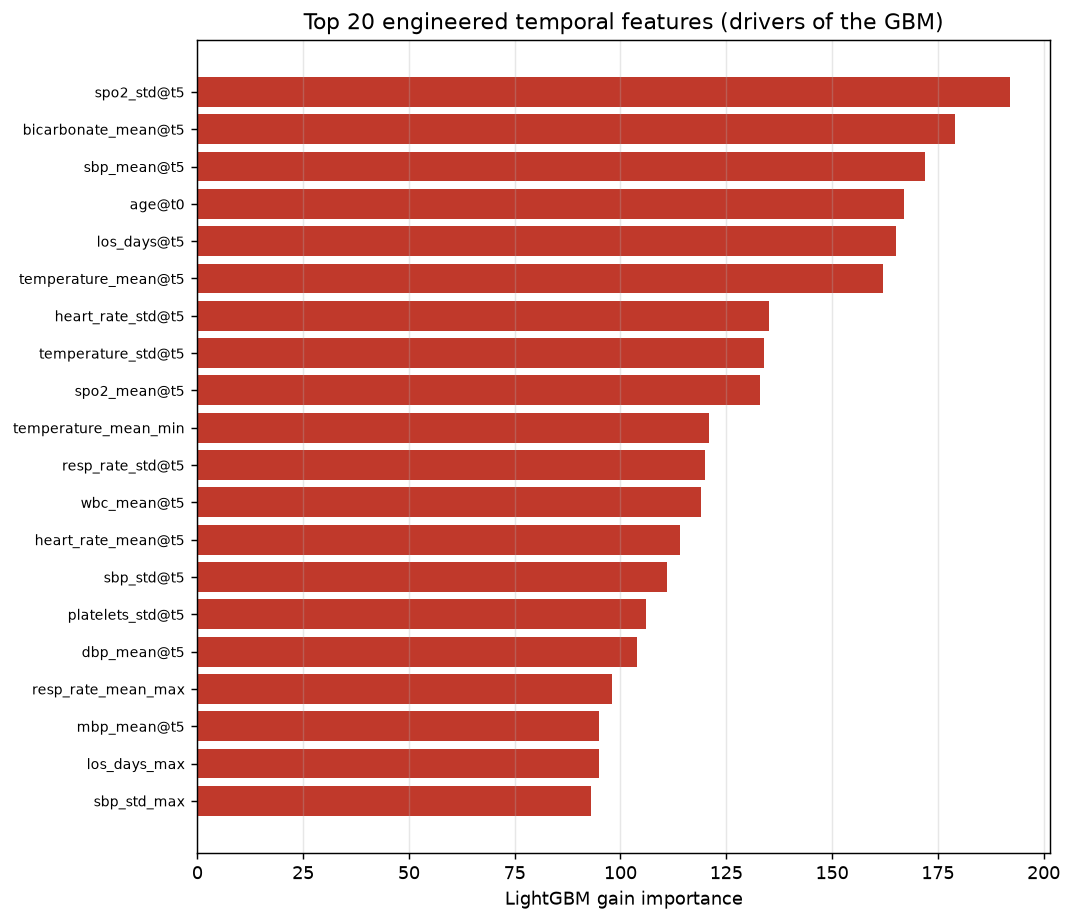
\includegraphics[width=0.49\columnwidth]{figures/improved_feature_importance.png}
\caption{Confusion matrix for the GBM soft-voting ensemble and leading LightGBM gain features.}
\label{fig:interpretability}
\end{figure}

\begin{figure}[t]
\centering
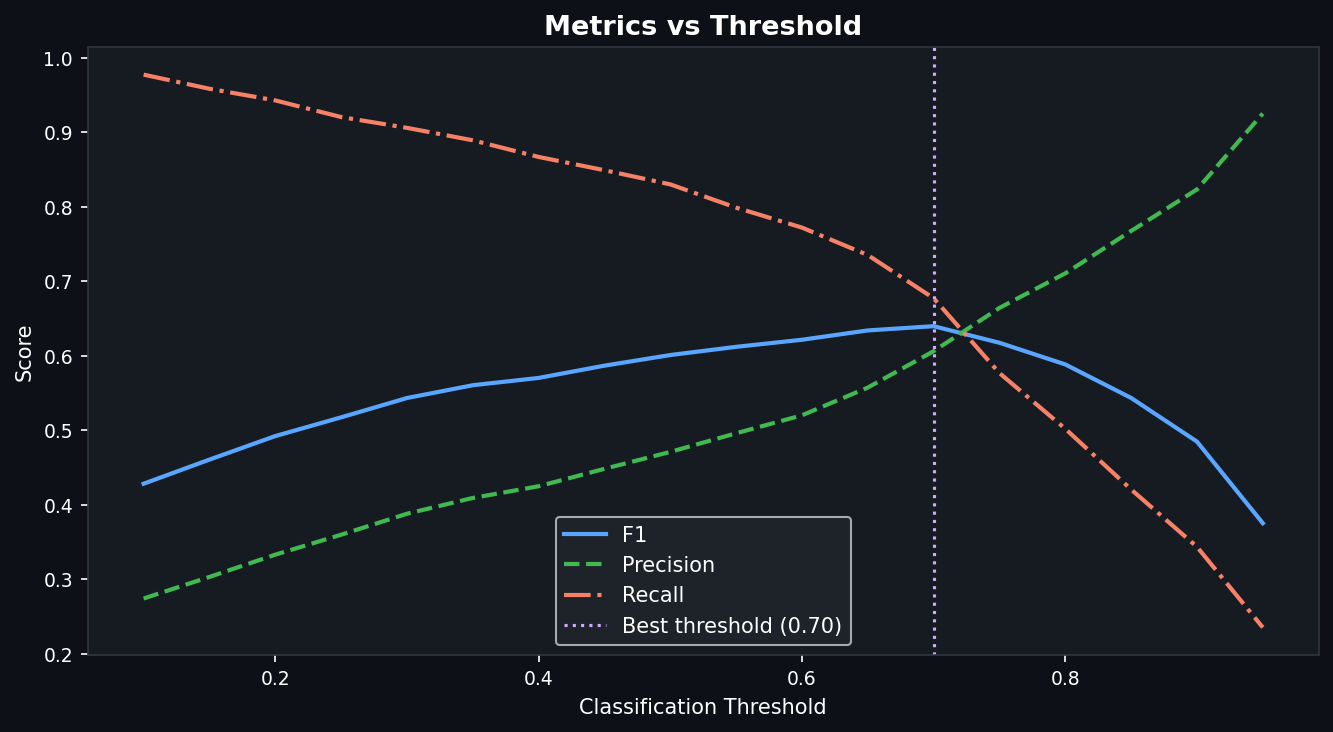
\includegraphics[width=0.9\columnwidth]{figures/lstm_threshold_sweep.png}
\caption{Example threshold sweep for an LSTM/BiLSTM model, illustrating the precision--recall tradeoff as the decision threshold varies.}
\label{fig:threshold}
\end{figure}

\section{Discussion}
For six-visit ICU trajectories, the dominant signal appears to be short-horizon change rather than long-range sequential dependence. Explicit deltas, slopes, velocities, accelerations, and variability statistics expose that structure to tree ensembles, which then model nonlinear interactions efficiently. Sequence models can in principle learn analogous representations, but under the present architecture, loss weighting, and fixed threshold of $0.5$, they favored recall over precision.

Calibration and threshold selection are first-class design choices~\cite{niculescu2005calibration}. Fig.~\ref{fig:threshold} illustrates how operating points move along the precision--recall frontier as the threshold changes. In any prospective decision-support setting, thresholds should be chosen against an explicit utility or workload constraint rather than F1 alone.

Deployment considerations also favor the boosting track in this study: the documented deployable artifact is approximately 3.3~MB and supports CPU inference without a deep-learning runtime~\cite{projectrepository}. That advantage is practical rather than clinical; compact artifacts do not imply bedside readiness.

\section{Limitations}
Several limitations constrain interpretation. First, evaluation is internal to one center's deidentified database and uses sample-level rather than patient-disjoint splits. Second, CSI is hand-engineered and not externally validated against clinician-adjudicated progression. Third, mortality fallback creates label heterogeneity between transitional and terminal samples. Fourth, missingness indicators are not yet explicit inputs, and medication-count features are proxy-derived. Fifth, subgroup performance by age, sex, race, admission type, and cardiac subtype is unreported. Sixth, statistical significance testing, calibration error, and multi-seed variability are not yet available. Seventh, improved deep-learning recipes and a proposed gated temporal attention network are documented in the project repository but lack finalized numbers in this manuscript~\cite{projectrepository}.
\textbf{[ABLATION EXPERIMENT REQUIRED: static vs.\ temporal features; CSI-only vs.\ mortality-fallback; patient-disjoint splits].}
\textbf{[BASELINE EXPERIMENT REQUIRED: logistic regression and random forest on the same temporal features].}

\section{Ethical and Data-Use Considerations}
MIMIC-IV is a deidentified critical-care database released through PhysioNet~\cite{johnson2023mimic,johnson2022mimiciv21}. Use requires credentialing and acceptance of the applicable data-use agreement. This paper reports a retrospective methodological study only. No IRB approval number is claimed here beyond the conditions attached to MIMIC-IV access, and the models are not approved for clinical use.

\section{Reproducibility}
Cohort construction, sequence building, model training, and visualization scripts are available in the project repository~\cite{projectrepository}. Raw MIMIC-IV files cannot be redistributed; credentialed users must obtain them from PhysioNet. Preprocessed arrays, random seeds for the reported stratified split, and evaluation scripts should be sufficient for re-training once local MIMIC access is configured.
\textbf{[IMPLEMENTATION DETAIL REQUIRED: pinned dependency versions / lockfile].}

\section{Conclusion}
This paper formulated longitudinal cardiac progression prediction on MIMIC-IV~2.1 six-visit ICU sequences and compared end-to-end sequence models with calibrated gradient boosting over engineered temporal descriptors. The reproduced Transformer baseline reached F1~$0.6319$ and ROC-AUC~$0.9168$; a soft-voting HistGradientBoosting--LightGBM--XGBoost ensemble reached F1~$0.7334$ and ROC-AUC~$0.9462$ on the same held-out test set. The results support the hypothesis that explicit short-horizon temporal structure can be more effective than larger sequence architectures for this task setting, subject to the stated leakage, label, and single-dataset limitations. Future work should enforce patient-disjoint chronological evaluation, validate labels clinically, report subgroup and calibration analyses, and complete pending deep-model experiments before any translational claim is considered.

\section*{Acknowledgment}
The authors thank the PhysioNet and MIMIC teams for providing deidentified critical-care data that enable reproducible clinical machine-learning research.

\bibliographystyle{IEEEtran}
\bibliography{references}

\end{document}
